\documentclass{article}
\usepackage[utf8]{inputenc}
\usepackage[T1]{fontenc}
\usepackage{lmodern}
\usepackage{graphicx}
\usepackage[frenchb]{babel}
\usepackage[table,xcdraw]{xcolor}
\usepackage{float}
\usepackage{fancyhdr}
\usepackage{geometry}
\usepackage{hyperref}

\newcommand{\info}{\texttt}
\newcommand{\pattern}{\emph}
\newcommand{\ue}{\textbf{X5I0010 "Objet et développement d'applications"}}

\title{Objet et développement d'applications - Design Patterns\\
Projet libre : \emph{BloodBowl}}
\author{Elbert Noel \bsc{Nyunting} \and Corentin \bsc{Chédotal}}
\date{19 Novembre 2016}

\geometry{hmargin=2cm,vmargin=3cm}

\pagestyle{fancy}
\fancyhf{}
\fancyhead[LE,RO]{Projet Blood Bowl 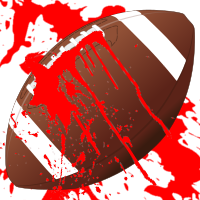
\includegraphics[width = 15px]{img/logo.png}}

\fancyfoot[LE,RO]{\thepage}

\begin{document}
\begin{titlepage}

\maketitle
\thispagestyle{empty}

\vspace{2cm}
\centerline{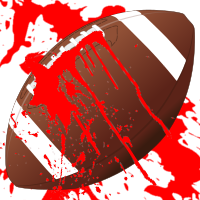
\includegraphics[scale=0.75]{img/logo.png}}
\vspace{2cm}

\begin{abstract}
    Dans le cadre de l'UE X5I0010 "Objet et développement d'applications" nous avons réalisé ce projet. Il comporte comme demandé plusieurs "designs patterns". Ont été utilisé les patterns \pattern{Strategy}, \pattern{State}, \pattern{Facade}, \pattern{Abstract Factory}. Ce rapport expliquera leur implémentation, le but et fonctionnement du projet ainsi que les difficultés rencontrées dans la réalisation de celui-ci.
\end{abstract}
\end{titlepage}

\newpage

\tableofcontents
\thispagestyle{empty}
\clearpage

\newpage

\pagenumbering{arabic}
\section{Introduction}
    
    L'Unité d'Enseignement \ue\ requérait la réalisation d'un projet de fin de semestre. Nous avions carte blanche dans le choix du sujet du projet (dans les limites du raisonnable bien sur). Notre binôme ayant un fort intérêt pour les jeux vidéos nous avons très tôt décidé de réaliser un prototype d'un jeu. Nous sommes partis sur de la stratégie au tour par tour car c'était le genre qui nous paraissait le plus réalisable dans le temps imparti tout en étant très ouvert aux différents patterns vus en cours. Enfin nous nous sommes raccrochés à une série de règles familière (BloodBowl) afin de ne pas perdre trop de temps dans le Game Design. Les règles ont cependant été évidemment adaptée au fonctionnement du programme\footnote{Les règles originales ainsi qu'une aide de jeu sont mises à disposition dans \info{/docs}} et pour permettre une inclusion plus facile des patterns.\\
    Très tôt dans la réalisation du projet il a été décidé de ne pas réaliser une interface graphique particulière. Toutes les interactions avec l'Utilisateur se faisant par le biais du terminal, à nouveau dans un but de gain de temps.

\section{Le projet}
    
    \emph{BloodBowl} est un jeu de plateau designé par \emph{Games Workshop}. Il voit deux équipes s'affronter dans un football américain déjanté et meurtrier, le tout dans un univers fantastique. Les joueurs jouent alors les coachs et gèrent leurs joueurs\footnote{A la suite de ce paragraphe on ne parlera plus que de "joueurs" pour désigner les personnages présents sur le terrain. Les joueurs humains seront eux appelés "coachs".} sur le terrain au tour par tour afin de marquer des "touchdowns". Notre projet est donc une réalisation de ce jeu sur terminal. Il est uniquement multijoueur et ne possède aucune intelligence artificielle contre laquelle jouer. De plus il n'est actuellement pas possible de créer son équipe à partir de rien, il faut sélectionner une équipe prédéfinie.\\
    Comme annoncé plus haut les interactions des joueurs avec le programme se font uniquement par le terminal et ainsi les action se font de façon textuelle. Un récapitulatif des commandes à disposition du joueur ainsi qu'une explication de l'interface graphique seront mise à disposition sur le Wiki du projet.\footnote{Disponible ici : \url{https://github.com/Heartbroken-Git/Project_Blood_Bowl/wiki}} 
    
    \subsection{Fonctionnement général}
        
        \begin{figure}[H]
            \centerline{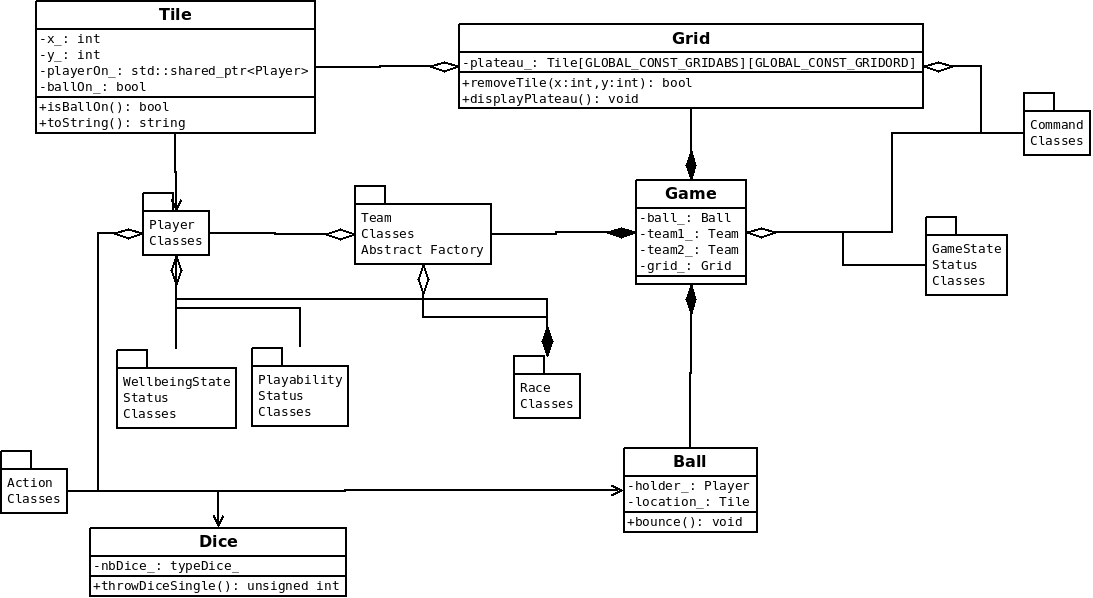
\includegraphics[scale=0.5]{img/UMLMain.png}}
            \caption{\label{DiaMain} Diagramme UML (simplifié) du projet}
        \end{figure}
        
        Le programme fonctionne autour de joueurs représentés par la classe Player et ses classes-filles. Ceux-ci sont posés sur des cases (Tile) elles-même composantes d'un plateau de jeu (Grid). Les joueurs ont différents états de santé et statuts représentés respectivement par Wellbeing et Playability. Les coachs vont demander tour à tour à leurs joueurs d'effectuer des actions en passant par la classe Commands, les actions spéciales réalisables par les joueurs sont dans la classe Action et ses classes-filles. De plus les joueurs composent une équipe d'une certaine race (humains, orcs ou elfes). Enfin Les classes Game, GameState, Ball et Dice servent au bon fonctionnement du jeu en tant que tel.

    \subsection{Principales classes (et classes filles associées)}
        
        La documentation Doxygen du projet est disponible pour les détails concernant le fonctionnement de chaque méthodes et le but de chaque attributs d'une classe donnée. Ainsi les paragraphes qui suit détailleront les fonctionnement et comportements des classes les plus importantes du projet sans nécessairement expliciter chaque opération effectuée.
        
        \subsubsection{Classe Player et Team}
        
            La classe Player représente les joueurs humains, orcs ou elfes composant les deux équipes. Elle a comme attributs les statistiques des joueurs, leurs noms et ainsi que leurs états de jouabilité \info{Playability} et santé \info{Wellbeing} qui changeront au cours de la partie si tout va bien. Ils ont ainsi des méthodes qui permet de vérifier si un joueur donné est encerclé ou non par des joueurs adverses, la distance entre deux joueurs, etc. Comme les Ogres, Trolls et Gobelins ne sont pas encore admis dans les match de Blood Bowl, les équipes humaines et orcs n'ont qu'accès aux quatre joueurs standards (Lineman, Blitzer, Catcher et Thrower) qui ont des statistiques différentes par rapport à leur races (les orcs sont plus robustes mais maladroit que les elfes qui eux sont plus habiles mais faibles que les humains, qui sont eux péniblement dans la moyenne.) Malheureusement, nous n'avons pas le temps de mettre en place un Team Editor et donc les coaches n'auront pas le plaisir de former leurs propres équipes ainsi que nommer ses joueurs. Ceci dit, nous avons mis des équipes prédéfinis pour chaque race suivant trois stratégies : équilibrée pour une équipe qui passe bien la balle et se défend bien, agile pour une équipe qui cherche à jouer le jeu et passer la balle et marquer le touchdown \textit{très} bien, et brute pour une équipe qui évite la balle et ne gagne qu'avec le fait que l'équipe adverse n'a plus de joueur sur le terrain. Ces stratégies sont indépendantes de la race, donc si pour une raison inconnue un coach décide de jouer avec une équipe elfe brute, il a tout à fait le droit. 
        
        \subsubsection{Classe Action}
        
            La grande cluster de classes Actions représente tout ce qu'un joueur peut faire dans la partie. De (tenter) passer le ballon à un camarade, (tenter) de bloquer un joueur adverse, et même (tenter) de taper sur un adversaire à terre sans se faire attraper par l'arbitre, Actions prend en compte tout ce qu'un joueur peut faire. Sauf de bouger, car nous avons décidé qu'un coach ne peut bouger son joueur une case à la fois (comme dans le jeu de plateau où les pions sont déplacés de cases en cases) et cela ne nécessite ni du pathfinding ni de calcul de coordonnées (comme ça c'est la faute du coach si un joueur entre dans un zone de tackle adverse.) Et chaque action est FINALE! Donc un joueur sélectionné perdra son tour si un autre joueur est sélectionné, même si le premier joueur n'a pas fait tous les actions qu'il peut faire. En effet, dans je jeu de plateau, un pion touché est un pion sélectionné et si on touche un autre pion, on ne peut plus jouer au pion précédent avant son prochain tour (c'est pour cela Blood Bowl se joue très peu parmi les jeunes d'aujourd'hui.)
        
        \subsubsection{Classes Grid et Tile}
        
            La classe \info{Grid} représente le plateau de jeu, composée de 26 sur 15 cases (appelée  \info{Tile} pour éviter de confondre avec le \info{case} de \info{switch}) dont une rangée de cases dans chaque représentant les lignes de touchdown. Tile contient ses coordonnées (en x et y), un booléen pour savoir si la balle est présent, et le joueur présent sur la case (ou pas, dans la plupart des cas.) Pour pouvoir mettre un joueur en \info{null} dans le cas où un joueur n'est pas sur la case, nous avons utilisé un \info{sharedptr} pointant vers un joueur. Enfin ces deux classes participent activement à l'affichage sauf dans le cas où un joueur serait présent sur la Tile auquel cas l'affichage est délégué à celui-ci.
        
        \subsubsection{Classe Commands}
            La classe \info{Commands} n'est qu'un simple pattern façade qui récupère les méthodes de la classe \info{Actions}, \info{Game},\info{Player} et \info{Team} et ne sert qu'à concaténer diverses actions et fonctionnements internes au programme afin de rendre une utilisation facile par le biais de commandes simples pour les coaches. 
        

    \subsection{Design patterns employés}
        
        Comme exigé dans le sujet nous avons fait appel à plus de 3 types de patterns différents et dans au moins deux familles (ici patterns de création et de comportement). Leur implémentation dans le projet est rapidement décrite ci-après.
        
        \subsubsection{Pattern \pattern{Strategy}}
            
            \begin{figure}[H]
                \centerline{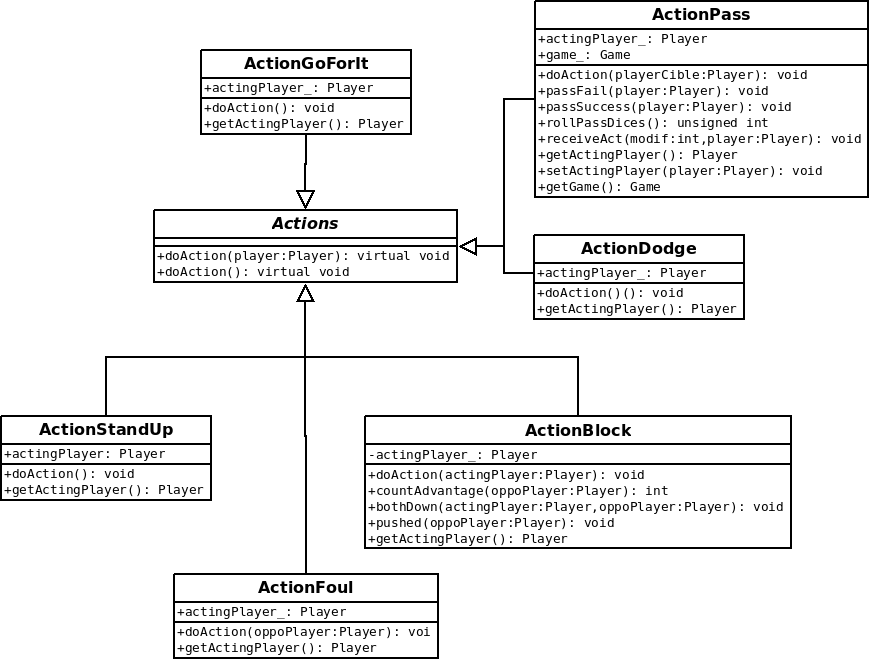
\includegraphics[scale=0.5]{img/Actions.png}}
                \caption{\label{DiaActions} Diagramme UML d'Action et de ses implémentations}
            \end{figure}
        
            Afin de modéliser les différentes actions que peut entreprendre un joueur nous avons décidé de se servir du pattern \pattern{Strategy}. En effet un joueur va réaliser "une" action, après quelle est-elle, comment fonctionne-t-elle exactement et sur quoi peut être et a donc été découplé par  l'utilisation de \pattern{Strategy}. On a donc un même appel initial qui suivant le choix de classes filles d'Action changera ce qui sera effectivement réalisé par le joueur.
        
        \subsubsection{Pattern \pattern{State}}
        
            \begin{figure}[H]
                \centerline{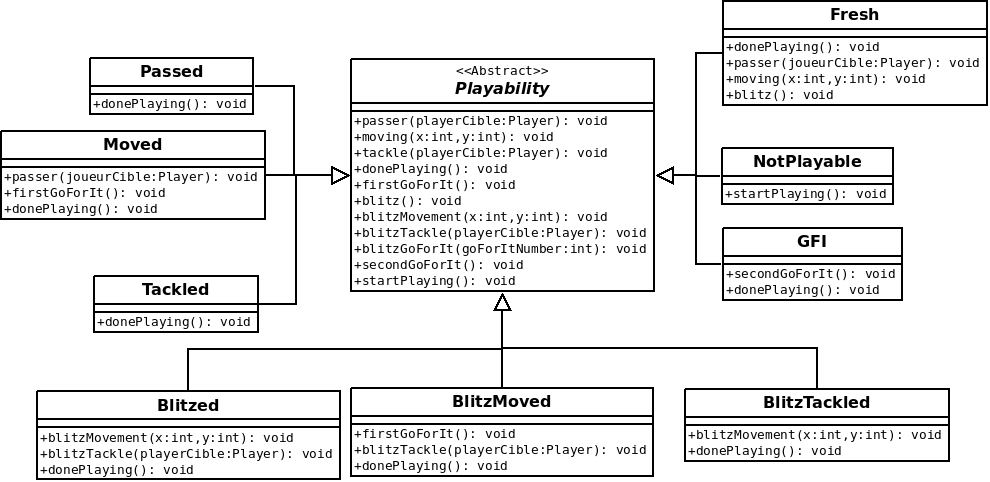
\includegraphics[scale=0.5]{img/PlayabilityState.png}}
                \caption{\label{DiaPlayability} Diagramme UML de Playability et de ses implémentations}
            \end{figure}
            
            Playability est un exemple de pattern \pattern{State} appliqué dans le projet. Celle-ci décrivant des statuts de jouabilité appliqués aux joueurs. Il était donc assez évident qu'un pattern \pattern{State} soit employé dans ce cas-là. Ainsi le code est maintenable et permet l'ajout ou le retrait de nouveaux statuts s'appliquant sur les joueurs. Les classes \info{Wellbeing} (état de santé des joueurs, indépendant, un peu, de leur jouabilité) et \info{GameState} (état du tour de jeu) utilisent aussi le \info{Pattern State} mais nous avons pris l'exemple de \info{Playability} car c'est le plus complexe et visuel des trois. Cependant il est à noté que les dimagrammes UML et d'états des autres classes sont disponibles en annexe \ref{annexe}.
        
        \subsubsection{Pattern \pattern{Abstract Factory}}
        
            \begin{figure}[H]
                \centerline{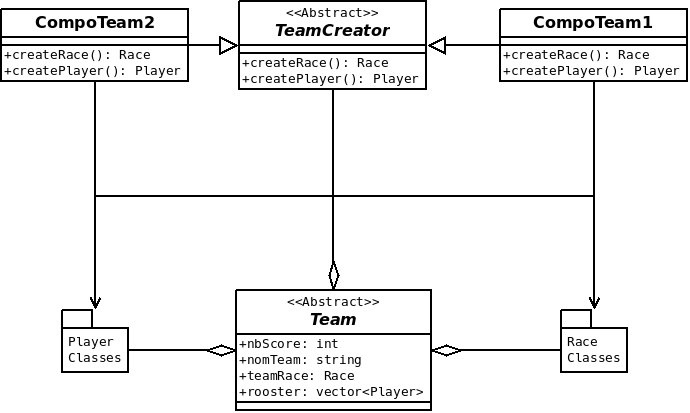
\includegraphics[scale=0.5]{img/Team.png}}
                \caption{\label{DiaTeam} Diagramme UML de Team et des classes associées}
            \end{figure}
        
            En toute honnêteté il est vrai que l'inclusion de ce pattern est un petit peu anti-naturelle. Malgré cela, il fallait trouver un autre pattern à employer et il ne nous semblait pas totalement idiot d'utiliser une \pattern{Factory} pour composer les équipes. Nous nous sommes reporté sur \pattern{Abstract Factory} car c'est le pattern qui nous semblait le plus compatible avec l'idée d'équipes précomposées (par exemple équipe agile, brute, ou équilibrée). Ainsi ce pattern nous permet de préparer les patrons des équipes, de quels types de joueurs elles doivent être composées et avec les trois races.
            
        \subsubsection{Pattern \pattern{Facade}}
            
            \begin{figure}[H]
                \centerline{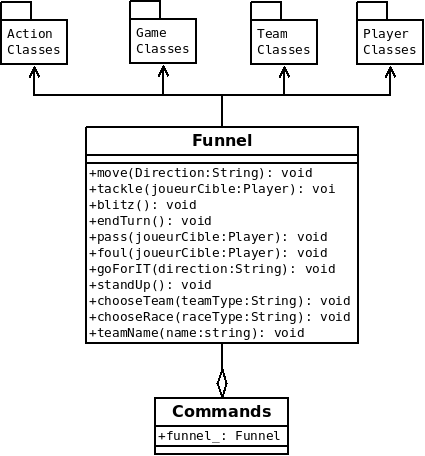
\includegraphics[scale=0.5]{img/Commands.png}}
                \caption{\label{DiaCommands} Diagramme UML de Commands et des classes associées}
            \end{figure}
            
            Afin de simplifier grandement l'utilisation du programme qui est déjà rendue quelque peu difficile par son aspect textuel nous avons décidé d'utiliser une \pattern{Facade}. Ainsi le coach rentre une commande, elle est interprétée et suivant celle-ci il suffit de n'appeler qu'une méthode qui va s'assurer de faire tous les appels dans les autres classes. Par exemple si un coach envoie la commande pour déplacer un joueur elle sera interprétée comme telle. Et la \pattern{Facade} déplacera le joueur d'une Tile à l'autre puis actualisera l'affichage pour refléter le mouvement. Tout ceci en exécutant finalement qu'une seule méthode et permettant un autre degré de découplage par rapport aux opérations effectuées en arrière plan.
 
 \section{Commentaires sur le projet}

    \subsection{La licence employée}
    
        Ce projet est purement universitaire et un défi pour nous même, une façon de pratiquer et de mieux apprendre les designs patterns mais aussi le C++. Se faisant nous ne voulions pas d'une licence restrictive car nous n'en voyions pas l'intérêt. Nous avons donc cherché une licence et celle qui initialement nous paraissait la plus compatible avec notre idée du projet était la \emph{MIT License}. Cependant au cours de nos recherches sur les licence libre nous sommes tombés sur la WTFPL. Malgré l'absence de clause de dégagement de responsabilité nous l'avons choisie car elle décrit finalement le mieux notre sentiment envers l'utilisation que d'autres pourraient faire de notre code écrit dans le cadre de ce projet.
    
    \subsection{Difficultés rencontrées}
    
        Le projet a fait face à quelques sévères difficultés durant son développement. Que ce soit des erreurs qui auraient pu être catastrophiques, la mise en place de nouveaux systèmes pas encore bien compris ou le temps passant très vite, les problèmes les plus importants que nous avons rencontrés sont explicités ci-dessous.
    
        \subsubsection{La \emph{Pushocalypse}}
        
            \info{Git} est un système de gestion de version particulièrement efficace et pratique. Nous l'avons utilisé dès la genèse du projet. Cependant tout produit puissant vient avec son lot de pièges et embûches. L'une d'entre elle la capacité de \info{git push -f} d'écraser l'arborescence du répertoire distant et de la remplacer par celle locale. Fonction qui peut être très pratique pour résoudre certains problèmes mais qui causa la suppression des modifications que l'un avait fait alors que l'autre fit un \info{git push -f} par mauvaise habitude alors qu'il n'avait pas récupéré les derniers commits en date avant. Fort heureusement une copie locale pré-\emph{Pushocalypse} put être récupérée et seulement deux petits commits durent être refait.
        
        \subsubsection{\info{Travis CI} ou comment je me suis battu pour mettre en place une belle-mère virtuelle}
        
            Afin de faciliter le débuggage et les test durant le développement surtout quand nous n'étions pas à travailler côte à côte. Il avait été décidé de mettre en place une intégration \info{Travis CI} très tôt dans le répertoire GitHub. Celui permettant alors d'avoir des logs précis, l'exécution de tests à chaque push sur la branche principale et le contrôle continu par \info{valgrind} contre d'éventuelles fuites mémoires.\\
            Seulement, aucun d'entre nous n'avait usé de \info{Travis} avant, or la réalisation du script \info{.travis.yml} ne fut pas la plus aisée. Elle prit une semaine par Corentin de bien mettre en place.
        
        \subsubsection{Débuggage des classes Action et Tile, la belle-mère contre attaque}
        
            La classe Action et ses sous-classes\dots\ Un élément primordial et principal de notre programme. Étant une classe qui gère les actions des joueurs des équipes, en utilisant les classes Ball et Dice, Elbert à très mal codé les classes pour commencer. Il s'est revendiqué en passant une semaine sur \info{Travis} (ou la belle mère) et débuggait les liens entre les classes différentes et fautes de frappes. Ensuite Elbert a débuggé la classe Tile, qui contient potentiellement un Player en attribut. N'étant pas sur Java, nous ne pouvons pas mettre un objet en NULL (cas où il n'y a pas de Player sur le Tile). Elbert a déduit qu'un pointeur est nécessaire, avec un Tile contenant un pointeur de Player. Il a ensuite déduit qu'il fallait utiliser un smart pointer\dots Un \info{unique\_ptr} . Après toute une journée avec la belle mère qui affichait des erreurs de compilations inconnues (ni par Elbert, ni par Corentin, ni par les M1 et M2 ALMA que nous connaissions) Elbert s'est rendu compte que \info{unique\_ptr} ne peut pas être égal à zéro. C'est pour cela que nous avons décidé d'utiliser \info{shared\_ptr} pour contenir les pointeurs de Player dans Tile. Une semaine et demi, près de 300 commits, et au moins une quarantaine de cafés noisettes plus tard, la belle mère affichait enfin zéro erreurs et nous laissait enfin mettre les classes de Action et Tile dans la branche master de notre git.
        
        \subsubsection{\bsc{Lamartine} serait fier de nous}
        
            Ce projet fut aussi l'occasion de nous rappeler combien le poète romantique avait raison. Le temps coule et même si nous cherchons à le remonter c'est impossible. En effet bien que très bien parti initialement nous avons très vite été rattrapé par les autres projets des autres UE et il est vite devenu difficile de gérer son temps. Nous avons donc fini acculé par celui-ci. Bien que nous n'avons pas l'impression d'avoir bâclé la réalisation du programme, il serait présomptueux que de dire que nous n'avons pas passé quelques longues nuits sur le projet afin de finir dans les temps. 
    
\section{Derniers mots}

    Ce fut un projet ardu et long. Si avec celui-ci nous n'avons pas chômé c'est tant mieux car en plus d'apprendre les designs patterns nous avons pu travailler d'autres aspects qui nous servirons dans le futur, au moins universitaire si ce n'est professionnel, tel que \info{Git}, \info{Travis CI} ou d'autres outils. Nous avons un peu plus approfondi nos connaissances du C++11 et gagné plus d'aisance avec celui-ci.\\
    De plus nous sommes tous les deux d'accord pour ne pas abandonner le projet de suite après sa remise. En effet nous avons tous les deux diverses fonctionnalités que nous aimerions intégrer par la suite. Fonctionnalités que nous avions du laisser tomber du fait du temps très limité, on compte ainsi par exemple la sauvegarde de données sur les équipes par fichiers XML la production de logs permettant de débriefer un match, éventuellement une AI rudimentaire, les autres équipes (sauf les nains, pas de nains tant qu'Elbert travaille encore sur ce projet), l'ajout de classes spéciales de joueurs\dots

\newpage
\appendix

\section{Annexe}

    \label{annexe}En annexe se trouve ci-après les diagrammes UML et diagrammes d'état des autres classes du projet qui n'ont été que survolées dans le rapport.

    \begin{figure}[H]
        \centerline{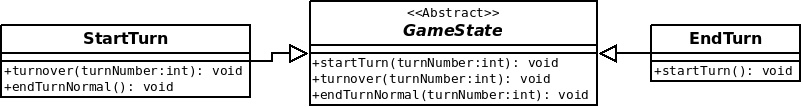
\includegraphics[scale=0.5]{img/GameState.png}}
        \caption{\label{DiaGameState} Diagramme UML de GameState et des classes associées}
    \end{figure}
    
    \begin{figure}[H]
        \centerline{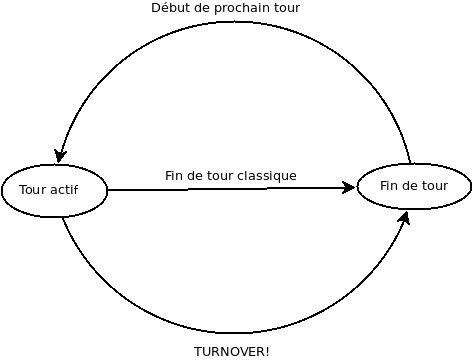
\includegraphics[scale=0.5]{img/GameStateGraph.png}}
        \caption{\label{DiaGameStateGraph} Diagramme d'état du jeu}
    \end{figure}
            
    \begin{figure}[H]
        \centerline{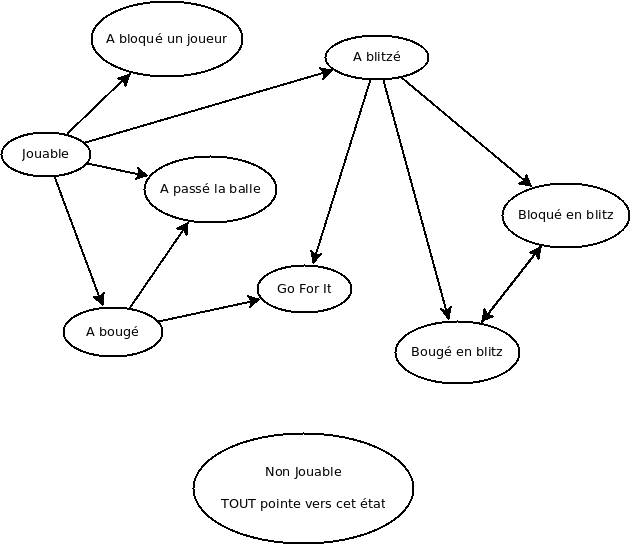
\includegraphics[scale=0.4]{img/PlayabilityGraph.png}}
        \caption{\label{DiaPlayabilityGraph} Diagramme d'état de la capacité d'un joueur à jouer}
    \end{figure}
            
    \begin{figure}[H]
        \centerline{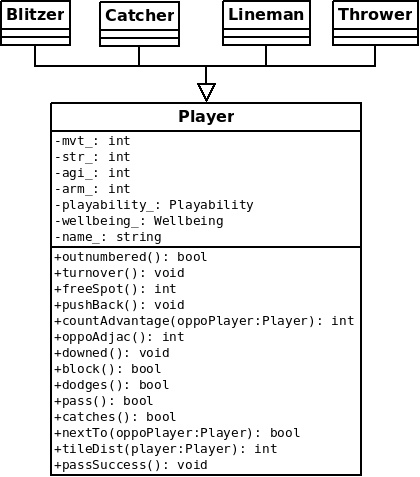
\includegraphics[scale=0.5]{img/Player.png}}
        \caption{\label{DiaPlayer} Diagramme UML de Player et de ses implémentations}
    \end{figure}
    
    \begin{figure}[H]
        \centerline{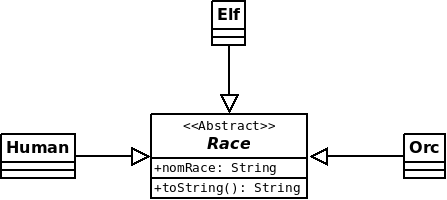
\includegraphics[scale=0.5]{img/Race.png}}
        \caption{\label{DiaRace} Diagramme UML de Race et de ses implémentations}
    \end{figure}
    
    \begin{figure}[H]
        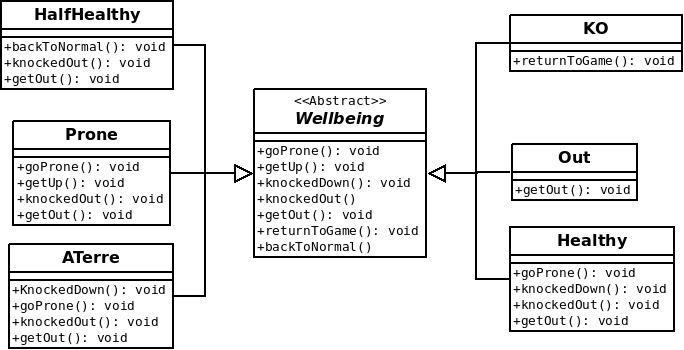
\includegraphics[scale=0.5]{img/WellbeingState.png}
        \caption{\label{DiaWellbeingState} Diagramme UML de Wellbeing et des classes associées}
    \end{figure}
    
    \begin{figure}[H]
        \centerline{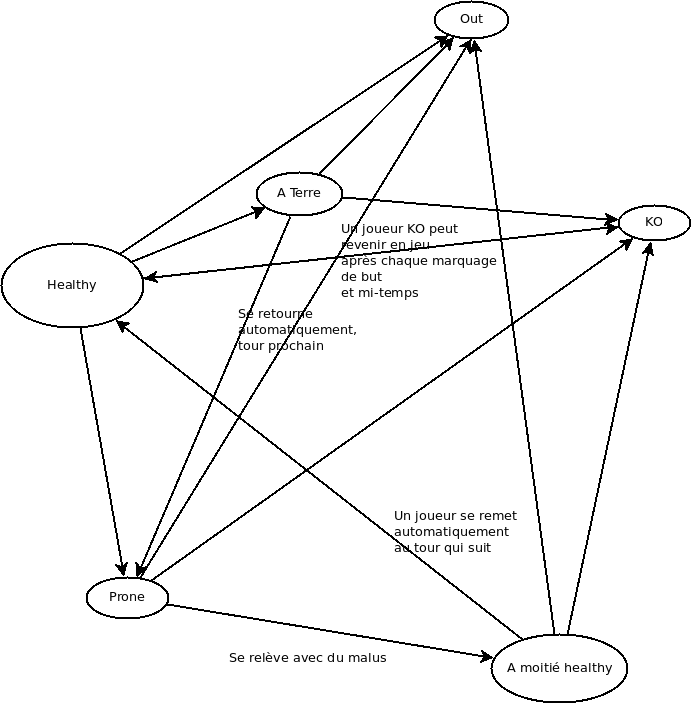
\includegraphics[scale=0.4]{img/WellbeingGraph.png}}
        \caption{\label{DiaWellbeingGraph} Diagramme d'état de l'état de santé d'un joueur}
    \end{figure}

\end{document}
